\section{Experiment 1: TransFuser with original ensemble of three sets of weights}
\label{sec:exp1}
In our first experiment, we evaluate TransFuser using a set of three pre-trained weights.

\subsection{Setup}
The pre-trained weights are downloaded from GitHub.\footnote{\url{https://github.com/autonomousvision/transfuser\#pretrained-agents}}
We use CARLA version 0.9.13 and our TransFuser code adapted to this version,
and run the evaluation script \texttt{docker/eval\_loop.sh}.


\subsection{Results}

The results from experiment 1 are shown in \cref{tab:exp1:results}.

We note that the logs from the output contained a warning that the evaluation was performed using a
Tesla Model 3 vehicle instead of the requested Lincoln MKZ 2017 vehicle.

\begin{table}[]
    \centering
    \begin{tabular}{|c|c|}
        \hline
        \textbf{Metric} & \textbf{Result} \\ \hline
        Routes completed & 30 / 36 \\ \hline
        Driving score & 6.84\% \\ \hline
        Route completion & 82.3\% \\ \hline
        Infraction penalty & 0.132 \\ \hline
        Collisions with pedestrians & 0.085 \\ \hline
        Collisions with vehicles & 7.3 \\ \hline
        Collisions with layout & 0.37 \\ \hline
        Red light infractions & 0.085 \\ \hline
        Stop sign infractions & 0.51 \\ \hline
        Off-road infractions & 0.37 \\ \hline
        Route deviations & 0.0 \\ \hline
        Route timeouts & 0.28 \\ \hline
        Agent blocked & 0.20 \\ \hline
    \end{tabular}
    \caption{Results from experiment 1. Infractions are given in counts per kilometer driven.}
    \label{tab:exp1:results}
\end{table}

We see that only 30 out of 36 routes in the Longest6 benchmark were completed.
The last 6 routes use the map called "Town06",
which was not present in our CARLA Docker environment,
thus the evaluation script was unable to load and evaluate these routes.

The remaining metrics are calculated as averages of the 
individual metrics on the 30 completed routes.
The various infractions are counts per kilometer driven.
We note a fairly high route completion score,
but unfortunately a severe infraction penalty
which causes the driving score to be very low.
By far the most common infraction is collision with other vehicles.

The locations of the various infractions can be seen in \cref{fig:exp1:town02}.
We note that most infractions occur in areas close to intersections or turns,
while the long straight road segments see almost no infractions.
A video of this experiment can be found here: \url{https://youtu.be/QyVsUrQynPU}. It contains the three
RGB cameras used as input to the model as well as an extra bird's-eye view used 
only for qualitative inspection.

\begin{figure}
    \centering
    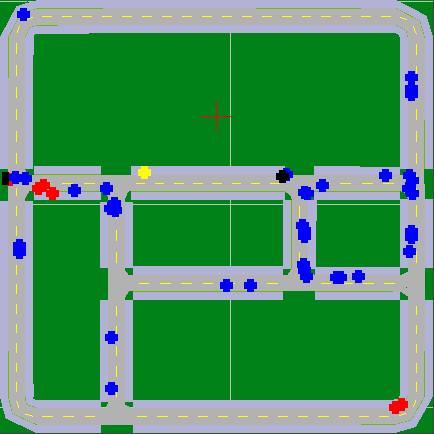
\includegraphics[width=0.5\textwidth]{chapters/4-experiments-results/figures/exp1-Town02.png}
    \caption{Infractions during experiment 1 on The town02 map.
    Red dots are collision with the scene geometry,
    and blue with other vehicles.
    The yellow dots indicate a red light infraction,
    and the black dots mark places where the agent was permanently blocked.}
    \label{fig:exp1:town02}
\end{figure}


\subsection{Discussion}

Due to the missing data for the last 6 routes,
we cannot claim an entirely valid comparison with this data and the results reported in \cite{transfuser-pami}.
However, it is unavoidable to see that the driving score is much lower than the $61.18\%$ reported on the CARLA Leaderboard. \todo{cite?}
The route completion score is similar to within a few percentage points,
thus the main reason is the infraction penalty which is a factor of 5 worse than the value reported on the CARLA Leaderboard.
Collision with vehicle infractions are the main cause of this penalty,
with a much higher count of $7.3$ per km compared to the online $0.81$ per km.

A possible reason for the increased collision count is the change of evaluation vehicle from
the Lincoln MKZ 2017 to the Tesla Model 3.
The vehicles may have different sizes and collision bounding boxes,
thus the agent may mistakenly assume that it has greater margins to other vehicles and the terrain
than it actually has.
The vehicles may also present different driving dynamics
which could further confuse the model.
We hypothesize that the model would perform better if evaluated using the correct vehicle,
and leave this evaluation for a future experiment.

As noted, the agent incurs most infractions in intersections or turns.
This indicates that these are difficult areas to navigate properly.
These areas require both keeping track of traffic signals,
reacting to other agents' behaviour,
and knowing the ego-agent's vehicle dynamics.
On the other hand,
straight segments only require the skill to keep proper spacing to the cars in front.
In our case even this skill isn't required,
since our model drives much slower than the surrounding traffic,
thus it will always have sufficient spacing in front to avoid collisions.
The exception is when other cars are standing still waiting in a queue,
in which case we do observe collisions,
for instance the ones seen to the top right in the figure.
This last behaviour is clearly present in the video as well,
where the model consistently fails to keep proper distance to vehicles in front.

On the other hand,
the video does indicate impressive compliance to red light signals.
The vehicle consistently stops when the signal is red,
and resumes driving when it changes to green.
However the agent is perhaps a bit pessimistic in how far away from the signal it stops,
it seems that the agent will stop as long as there is a red light in view,
no matter how far away.
This could in-fact be a behaviour learned from the expert agent,
which we have not investigated.
Future experiments should therefore perform both quantitative and qualitative
evaluations of the expert agent to find the upper bound on the imitating agent's potential.
